% ════════════════════════════════════════════════════════════════════════════
% FINANCEFLOW - BEAMER PRESENTATION
% ════════════════════════════════════════════════════════════════════════════
% A professional Beamer presentation for the FinanceFlow project
% Created: April 2026
% Document Class: Beamer (16:9 aspect ratio, 12pt font)
% ════════════════════════════════════════════════════════════════════════════

\documentclass[aspectratio=169, 12pt]{beamer}

% ────────────────────────────────────────────────────────────────────────────
% BEAMER THEME CONFIGURATION
% ────────────────────────────────────────────────────────────────────────────
\usetheme{default}
\usecolortheme{default}

% ────────────────────────────────────────────────────────────────────────────
% PACKAGE IMPORTS
% ────────────────────────────────────────────────────────────────────────────
\usepackage[utf8]{inputenc}        % UTF-8 input encoding
\usepackage[T1]{fontenc}            % T1 font encoding
\usepackage{lmodern}                % Latin Modern fonts
\usepackage{tikz}                   % For diagrams and graphics
\usepackage{booktabs}               % Professional tables
\usepackage{tabularx}               % Extended table functionality
\usepackage{listings}               % Code listings
\usepackage{multicol}               % Multiple columns
\usepackage{array}                  % Enhanced arrays and tables

% ────────────────────────────────────────────────────────────────────────────
% COLOR DEFINITIONS
% ────────────────────────────────────────────────────────────────────────────
% Brand colors for FinanceFlow
\definecolor{primary}{HTML}{0D968B}     % Teal - Primary brand color
\definecolor{darkbg}{HTML}{0F1F1D}      % Dark background for title slides
\definecolor{accent}{HTML}{2563EB}      % Blue - Accent color
\definecolor{lightbg}{HTML}{F0FAF9}     % Light background for blocks
\definecolor{codebg}{HTML}{E8F5F3}      % Code background
\definecolor{warn}{HTML}{F59E0B}        % Warning/highlight color

% ────────────────────────────────────────────────────────────────────────────
% BEAMER COLOR THEME CUSTOMIZATION
% ────────────────────────────────────────────────────────────────────────────
% Palette colors
\setbeamercolor{palette primary}{bg=primary, fg=white}
\setbeamercolor{palette secondary}{bg=darkbg, fg=white}

% Title slide colors
\setbeamercolor{title}{fg=white}
\setbeamercolor{subtitle}{fg=primary!30!white}

% Frame title colors
\setbeamercolor{frametitle}{fg=primary, bg=white}
\setbeamercolor{normal text}{fg=darkbg}

% List item colors
\setbeamercolor{item}{fg=primary}

% Block colors (for callout boxes)
\setbeamercolor{block title}{bg=primary, fg=white}
\setbeamercolor{block body}{bg=lightbg, fg=darkbg}
\setbeamercolor{block title alerted}{bg=red!70!black, fg=white}
\setbeamercolor{block body alerted}{bg=red!5, fg=darkbg}
\setbeamercolor{block title example}{bg=accent, fg=white}
\setbeamercolor{block body example}{bg=accent!5, fg=darkbg}

% ────────────────────────────────────────────────────────────────────────────
% BEAMER TEMPLATE CUSTOMIZATION
% ────────────────────────────────────────────────────────────────────────────
% Remove navigation symbols
\setbeamertemplate{navigation symbols}{}

% Custom footer with slide numbers
\setbeamertemplate{footline}{
    \hfill\textcolor{gray!60}{\insertframenumber/\inserttotalframenumber}\hspace{12pt}\vspace{6pt}
}

% Custom frame title with underline
\setbeamertemplate{frametitle}{
    \vspace{6pt}
    {\large\bfseries\insertframetitle}
    \ifx\insertframesubtitle\empty\else
        \\[2pt]{\small\color{gray}\insertframesubtitle}
    \fi
    \vspace{-2pt}
    \textcolor{primary}{\rule{\textwidth}{1.5pt}}
    \vspace{4pt}
}

% Item markers
\setbeamertemplate{itemize items}[circle]
\setbeamertemplate{enumerate items}[default]

% ────────────────────────────────────────────────────────────────────────────
% FONT CUSTOMIZATION
% ────────────────────────────────────────────────────────────────────────────
\setbeamerfont{title}{size=\Huge, series=\bfseries}
\setbeamerfont{subtitle}{size=\large}
\setbeamerfont{frametitle}{size=\large, series=\bfseries}

% ────────────────────────────────────────────────────────────────────────────
% CODE LISTING SETTINGS
% ────────────────────────────────────────────────────────────────────────────
\lstset{
    basicstyle=\scriptsize\ttfamily,
    backgroundcolor=\color{codebg},
    frame=none,
    breaklines=true,
    xleftmargin=4pt,
    xrightmargin=4pt,
}

% ────────────────────────────────────────────────────────────────────────────
% PRESENTATION METADATA
% ────────────────────────────────────────────────────────────────────────────
\title{FinanceFlow}
\subtitle{Personal Finance Management Application}
\author{Web Programming Project}
\date{April 2026}

% ════════════════════════════════════════════════════════════════════════════
% DOCUMENT BEGINS HERE
% ════════════════════════════════════════════════════════════════════════════
\begin{document}

% ════════════════════════════════════════════════════════════════════════════
% SECTION 1: TITLE SLIDE
% ════════════════════════════════════════════════════════════════════════════
{
\setbeamercolor{background canvas}{bg=darkbg}
\begin{frame}[plain]
\begin{center}
\vspace{1.5cm}
{\Huge\bfseries\textcolor{primary}{FinanceFlow}}\par
\vspace{8pt}
{\large\textcolor{white}{Personal Finance Management Application}}\par
\vspace{6pt}
{\small\textcolor{gray!50}{A Modern Full-Stack Web Application}}\par
\vspace{1.2cm}
\textcolor{primary}{\rule{0.4\textwidth}{2pt}}\par
\vspace{1.2cm}
{\normalsize\textcolor{white}{Web Programming Project}}\par
\vspace{8pt}
{\small\textcolor{gray!50}{Node.js \,|\, Express.js \,|\, MySQL/PostgreSQL \,|\, Vanilla JavaScript}}\par
\vspace{8pt}
{\small\textcolor{gray!60}{April 2026}}\par
\end{center}
\end{frame}
}

% ════════════════════════════════════════════════════════════════════════════
% SECTION 2: AGENDA
% ════════════════════════════════════════════════════════════════════════════
\begin{frame}{Agenda}
\begin{enumerate}\itemsep=10pt
    \item Project Overview
    \item \textbf{Front-End} --- What \& Why
    \item \textbf{Back-End} --- What \& Why
    \item \textbf{Database} --- What \& Why
    \item System Architecture
    \item Database Schema
    \item API Design
    \item Key Features
    \item Security
    \item Deployment
    \item Tech Stack Summary
\end{enumerate}
\end{frame}

% ════════════════════════════════════════════════════════════════════════════
% SECTION 3: PROJECT OVERVIEW
% ════════════════════════════════════════════════════════════════════════════
\begin{frame}{Project Overview}
\textbf{FinanceFlow} is a full-stack personal finance app for tracking income, managing expenses, setting savings goals, and gaining financial insights.

\vspace{10pt}
\begin{columns}[T]
\begin{column}{0.48\textwidth}
\begin{block}{Core Features}
\begin{itemize}\itemsep=2pt
    \item Real-time dashboard with charts
    \item Income \& expense CRUD
    \item Savings goals with progress
    \item Analytics \& health score
\end{itemize}
\end{block}
\end{column}
\begin{column}{0.48\textwidth}
\begin{block}{Highlights}
\begin{itemize}\itemsep=2pt
    \item Multi-currency (INR, USD, EUR, GBP)
    \item Dark/light mode
    \item Responsive (mobile-first)
    \item Zero-config startup
\end{itemize}
\end{block}
\end{column}
\end{columns}
\end{frame}

% ════════════════════════════════════════════════════════════════════════════
% SECTION 4: FRONTEND TECHNOLOGY
% ════════════════════════════════════════════════════════════════════════════

% ────────────────────────────────────────────────────────────────────────────
% SLIDE 4A: Front-End - What Technologies Are Used?
% ────────────────────────────────────────────────────────────────────────────
\begin{frame}{Front-End Technology}
\framesubtitle{What is used?}

\begin{center}
\begin{tabular}{l l l}
\toprule
\textbf{Technology} & \textbf{Version} & \textbf{Role} \\
\midrule
Vanilla JavaScript & ES6+ & Application logic \\
Tailwind CSS & CDN (latest) & Utility-first styling \\
Chart.js & CDN (latest) & Financial visualizations \\
Material Symbols & CDN & Icons \\
Google Fonts (Inter) & CDN & Typography \\
\bottomrule
\end{tabular}
\end{center}

\vspace{10pt}
\begin{block}{Architecture}
\textbf{Multi-Page Application (MPA)} --- each page is a self-contained HTML file with embedded JS. No build tools, no bundlers, no \texttt{node\_modules} on the frontend.
\end{block}
\end{frame}

% ────────────────────────────────────────────────────────────────────────────
% SLIDE 4B: Front-End - Why These Choices?
% ────────────────────────────────────────────────────────────────────────────
\begin{frame}{Front-End --- Why These Choices?}

\begin{columns}[T]
\begin{column}{0.48\textwidth}
\begin{block}{Why Vanilla JS?}
\begin{itemize}\itemsep=2pt
    \item \textbf{Zero build step} --- no Webpack/Vite needed
    \item \textbf{No dependency overhead} --- instant loading
    \item \textbf{Simpler debugging} --- no framework abstractions
    \item \textbf{Direct deployment} --- static files on Vercel
    \item Modern ES6+: async/await, modules, destructuring
\end{itemize}
\end{block}
\end{column}
\begin{column}{0.48\textwidth}
\begin{block}{Why Tailwind CSS?}
\begin{itemize}\itemsep=2pt
    \item \textbf{Utility-first} --- rapid UI development
    \item \textbf{Responsive} built-in (sm/md/lg)
    \item \textbf{Dark mode} --- native class-based toggle
    \item Plugins: \texttt{forms}, \texttt{container-queries}
\end{itemize}
\end{block}
\vspace{4pt}
\begin{block}{Why Chart.js?}
\begin{itemize}\itemsep=2pt
    \item Simple API for bar/donut/line charts
    \item Interactive tooltips \& animations
    \item Responsive \& lightweight
\end{itemize}
\end{block}
\end{column}
\end{columns}
\end{frame}

% ════════════════════════════════════════════════════════════════════════════
% SECTION 5: BACKEND TECHNOLOGY
% ════════════════════════════════════════════════════════════════════════════

% ────────────────────────────────────────────────────────────────────────────
% SLIDE 5A: Back-End - What Technologies Are Used?
% ────────────────────────────────────────────────────────────────────────────
\begin{frame}{Back-End Technology}
\framesubtitle{What is used?}

\begin{center}
\begin{tabular}{l l l}
\toprule
\textbf{Technology} & \textbf{Version} & \textbf{Role} \\
\midrule
Node.js & 18+ & Server runtime \\
Express.js & v5.2 & Web framework / REST API \\
TypeScript & v5.6 (partial) & Type-safe services \& routes \\
Helmet & v8.1 & Security HTTP headers \\
CORS & v2.8 & Cross-origin access \\
express-rate-limit & v8.3 & API rate limiting \\
compression & v1.8 & gzip response compression \\
dotenv & v16.6 & Environment configuration \\
\bottomrule
\end{tabular}
\end{center}
\end{frame}

% ────────────────────────────────────────────────────────────────────────────
% SLIDE 5B: Back-End - Why These Choices?
% ────────────────────────────────────────────────────────────────────────────
\begin{frame}{Back-End --- Why These Choices?}

\begin{columns}[T]
\begin{column}{0.48\textwidth}
\begin{block}{Why Node.js?}
\begin{itemize}\itemsep=2pt
    \item \textbf{JS everywhere} --- same language front \& back
    \item \textbf{Non-blocking I/O} --- handles concurrent requests
    \item \textbf{npm ecosystem} --- largest package registry
    \item \textbf{Vercel-native} --- first-class serverless support
    \item ES Modules throughout
\end{itemize}
\end{block}
\end{column}
\begin{column}{0.48\textwidth}
\begin{block}{Why Express.js v5?}
\begin{itemize}\itemsep=2pt
    \item \textbf{Minimal \& flexible} --- unopinionated
    \item \textbf{Industry standard} --- massive community
    \item \textbf{Middleware pipeline} --- composable layers
    \item \textbf{Easy REST APIs} --- simple route definitions
    \item v5: native async error handling
\end{itemize}
\end{block}
\end{column}
\end{columns}

\vspace{8pt}
\begin{block}{Security Stack}
\textbf{Helmet} (secure headers) + \textbf{CORS} (cross-origin) + \textbf{rate-limit} (abuse prevention) + \textbf{compression} (bandwidth)
\end{block}
\end{frame}

% ════════════════════════════════════════════════════════════════════════════
% SECTION 6: DATABASE TECHNOLOGY
% ════════════════════════════════════════════════════════════════════════════

% ────────────────────────────────────────────────────────────────────────────
% SLIDE 6A: Database - What Technologies Are Used?
% ────────────────────────────────────────────────────────────────────────────
\begin{frame}{Database Technology}
\framesubtitle{What is used?}

\begin{center}
\begin{tabular}{l l l}
\toprule
\textbf{Technology} & \textbf{Driver} & \textbf{Role} \\
\midrule
MySQL 8 & mysql2 v3.20 & Local/self-hosted database \\
PostgreSQL & pg v8.16 & Cloud database (Neon) \\
In-Memory (JS) & --- & Zero-config fallback \\
\bottomrule
\end{tabular}
\end{center}

\vspace{8pt}
\begin{block}{Auto-Detection}
The \texttt{connection.mjs} module inspects \texttt{DATABASE\_URL}:
\begin{itemize}\itemsep=1pt
    \item \texttt{postgres://...} $\rightarrow$ PostgreSQL mode
    \item \texttt{mysql://...} or discrete \texttt{DB\_*} vars $\rightarrow$ MySQL mode
    \item No config $\rightarrow$ In-memory fallback
\end{itemize}
A translation layer converts MySQL \texttt{?} placeholders to PostgreSQL \texttt{\$1, \$2} automatically.
\end{block}
\end{frame}

% ────────────────────────────────────────────────────────────────────────────
% SLIDE 6B: Database - Why These Choices?
% ────────────────────────────────────────────────────────────────────────────
\begin{frame}{Database --- Why These Choices?}

\begin{columns}[T]
\begin{column}{0.32\textwidth}
\begin{block}{Why MySQL?}
\begin{itemize}\itemsep=2pt
    \item Widely used \& documented
    \item ACID compliant
    \item InnoDB: FK + crash recovery
    \item Easy local setup
\end{itemize}
\end{block}
\end{column}
\begin{column}{0.32\textwidth}
\begin{block}{Why PostgreSQL?}
\begin{itemize}\itemsep=2pt
    \item Cloud-native (Neon on Vercel)
    \item Production-grade optimizer
    \item Free tier available
    \item Advanced features
\end{itemize}
\end{block}
\end{column}
\begin{column}{0.32\textwidth}
\begin{block}{Why No ORM?}
\begin{itemize}\itemsep=2pt
    \item Full SQL control
    \item Parameterized queries prevent injection
    \item No hidden magic
    \item Zero overhead
\end{itemize}
\end{block}
\end{column}
\end{columns}

\vspace{8pt}
\begin{exampleblock}{Why Dual Support?}
\textbf{Flexibility} --- MySQL for local development, PostgreSQL (Neon) for cloud/Vercel production. No vendor lock-in.
\end{exampleblock}
\end{frame}

% ════════════════════════════════════════════════════════════════════════════
% SECTION 7: SYSTEM ARCHITECTURE
% ════════════════════════════════════════════════════════════════════════════
\begin{frame}{System Architecture}

\begin{center}
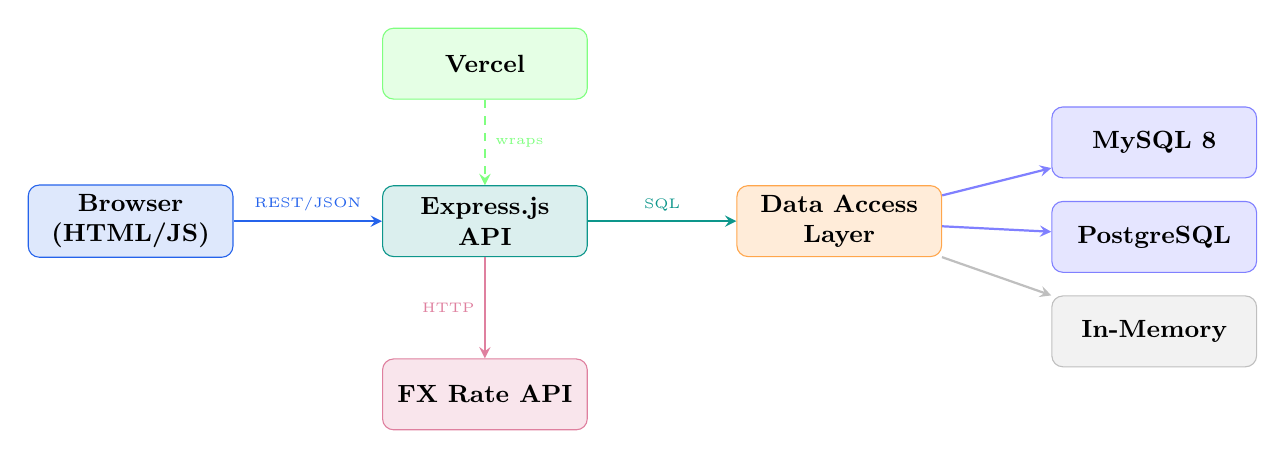
\begin{tikzpicture}[
    box/.style={draw, rounded corners=4pt, minimum width=2.6cm, minimum height=0.9cm, align=center, font=\small\bfseries},
    arrow/.style={->, thick, >=stealth},
    lbl/.style={font=\tiny\color{gray}, align=center}
]

% Client and server nodes
\node[box, fill=accent!15, draw=accent] (client) at (0, 0) {Browser\\(HTML/JS)};
\node[box, fill=primary!15, draw=primary] (api) at (4.5, 0) {Express.js\\API};
\node[box, fill=orange!15, draw=orange!70] (dal) at (9, 0) {Data Access\\Layer};

% Database nodes
\node[box, fill=blue!10, draw=blue!50] (mysql) at (13, 1) {MySQL 8};
\node[box, fill=blue!10, draw=blue!50] (pg) at (13, -0.2) {PostgreSQL};
\node[box, fill=gray!10, draw=gray!50] (mem) at (13, -1.4) {In-Memory};

% External services
\node[box, fill=purple!10, draw=purple!50] (fx) at (4.5, -2.2) {FX Rate API};
\node[box, fill=green!10, draw=green!50] (vercel) at (4.5, 2) {Vercel};

% Arrows showing data flow
\draw[arrow, accent] (client) -- node[above, lbl] {REST/JSON} (api);
\draw[arrow, primary] (api) -- node[above, lbl] {SQL} (dal);
\draw[arrow, blue!50] (dal) -- (mysql);
\draw[arrow, blue!50] (dal) -- (pg);
\draw[arrow, gray!50] (dal) -- (mem);
\draw[arrow, purple!50] (api) -- node[left, lbl] {HTTP} (fx);
\draw[arrow, green!50, dashed] (vercel) -- node[right, lbl] {wraps} (api);

\end{tikzpicture}
\end{center}
\end{frame}

% ════════════════════════════════════════════════════════════════════════════
% SECTION 8: DATABASE SCHEMA
% ════════════════════════════════════════════════════════════════════════════
\begin{frame}{Database Schema}
\framesubtitle{4 core tables with foreign key relationships}

\begin{center}
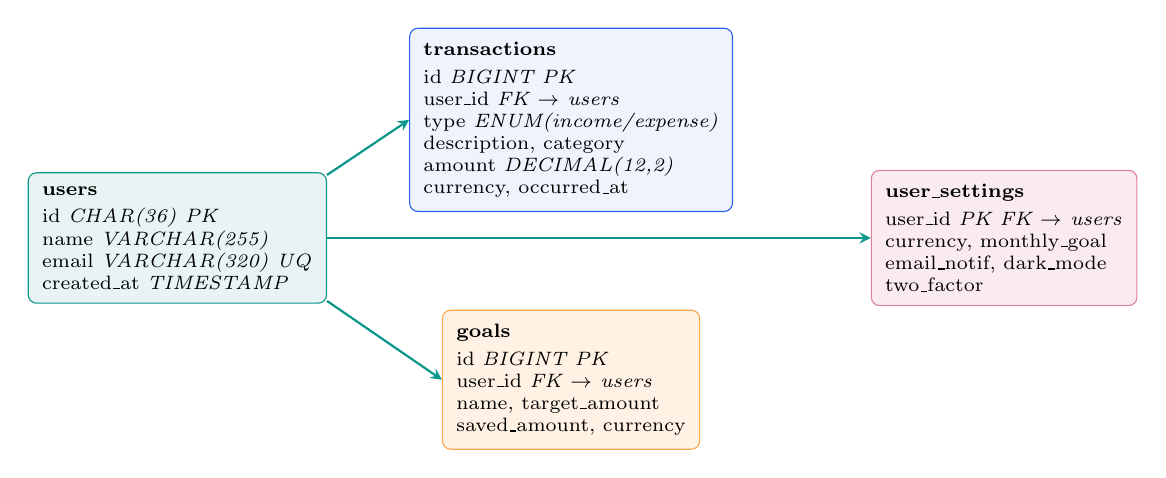
\begin{tikzpicture}[
    table/.style={draw, rounded corners=3pt, minimum width=3cm, align=left, font=\scriptsize, inner sep=5pt},
    title/.style={font=\scriptsize\bfseries\color{white}},
    arrow/.style={->, thick, >=stealth, primary}
]

% Users table (central hub)
\node[table, fill=primary!10, draw=primary] (users) at (0, 0) {
    \textbf{users}\\[2pt]
    id \textit{CHAR(36) PK}\\
    name \textit{VARCHAR(255)}\\
    email \textit{VARCHAR(320) UQ}\\
    created\_at \textit{TIMESTAMP}
};

% Transactions table (foreign key to users)
\node[table, fill=accent!8, draw=accent] (txns) at (5, 1.5) {
    \textbf{transactions}\\[2pt]
    id \textit{BIGINT PK}\\
    user\_id \textit{FK $\rightarrow$ users}\\
    type \textit{ENUM(income/expense)}\\
    description, category\\
    amount \textit{DECIMAL(12,2)}\\
    currency, occurred\_at
};

% Goals table (foreign key to users)
\node[table, fill=orange!10, draw=orange!70] (goals) at (5, -1.8) {
    \textbf{goals}\\[2pt]
    id \textit{BIGINT PK}\\
    user\_id \textit{FK $\rightarrow$ users}\\
    name, target\_amount\\
    saved\_amount, currency
};

% Settings table (foreign key to users)
\node[table, fill=purple!8, draw=purple!50] (settings) at (10.5, 0) {
    \textbf{user\_settings}\\[2pt]
    user\_id \textit{PK FK $\rightarrow$ users}\\
    currency, monthly\_goal\\
    email\_notif, dark\_mode\\
    two\_factor
};

% Foreign key relationships
\draw[arrow] (users.east) ++(0, 0.8) -- (txns.west);
\draw[arrow] (users.east) ++(0, -0.8) -- (goals.west);
\draw[arrow] (users.east) -- (settings.west);

\end{tikzpicture}
\end{center}

\vspace{4pt}
\begin{center}
\small All foreign keys use \textbf{ON DELETE CASCADE} for referential integrity.
\end{center}
\end{frame}

% ════════════════════════════════════════════════════════════════════════════
% SECTION 9: REST API DESIGN
% ════════════════════════════════════════════════════════════════════════════
\begin{frame}{REST API Endpoints}

\begin{center}
\scriptsize
\begin{tabular}{l l l}
\toprule
\textbf{Method} & \textbf{Endpoint} & \textbf{Description} \\
\midrule
\multicolumn{3}{l}{\textit{\textcolor{primary}{Authentication}}} \\
POST & /api/auth/login & Login \\
POST & /api/auth/signup & Register \\
\midrule
\multicolumn{3}{l}{\textit{\textcolor{primary}{Dashboard \& Analytics}}} \\
GET & /api/dashboard & Dashboard stats, goals, recent txns \\
GET & /api/analytics & Monthly trends, category breakdown \\
\midrule
\multicolumn{3}{l}{\textit{\textcolor{primary}{Transactions}}} \\
GET & /api/transactions & List (filter: type, category, search) \\
POST & /api/transactions & Create transaction \\
PUT & /api/transactions/:id & Update transaction \\
DELETE & /api/transactions/:id & Delete transaction \\
\midrule
\multicolumn{3}{l}{\textit{\textcolor{primary}{Goals \& Settings}}} \\
GET/POST/PUT/DELETE & /api/goals & Full CRUD for savings goals \\
GET/PUT & /api/settings & User preferences \\
GET & /api/fx/latest & FX rates (6h cached) \\
\bottomrule
\end{tabular}
\end{center}
\end{frame}

% ════════════════════════════════════════════════════════════════════════════
% SECTION 10: KEY FEATURES
% ════════════════════════════════════════════════════════════════════════════
\begin{frame}{Key Features}

\begin{columns}[T]
\begin{column}{0.48\textwidth}

\begin{block}{Dashboard}
\begin{itemize}\itemsep=1pt
    \item Total income, expenses, balance
    \item Savings rate percentage
    \item Financial Health Score (0--100)
    \item Interactive Chart.js visualizations
    \item Recent transactions
\end{itemize}
\end{block}

\begin{block}{Income \& Expenses}
\begin{itemize}\itemsep=1pt
    \item Full CRUD operations
    \item Category filtering \& search
    \item Pagination (10/page)
    \item Monthly totals \& trends
\end{itemize}
\end{block}

\end{column}
\begin{column}{0.48\textwidth}

\begin{block}{Analytics}
\begin{itemize}\itemsep=1pt
    \item Weekly/monthly trends
    \item Category breakdown charts
    \item Income vs expense comparison
    \item Financial health insights
\end{itemize}
\end{block}

\begin{block}{User Experience}
\begin{itemize}\itemsep=1pt
    \item Dark/light mode toggle
    \item Responsive (mobile-first)
    \item Multi-currency (INR/USD/EUR/GBP)
    \item Toast notifications
    \item Custom modal system
\end{itemize}
\end{block}

\end{column}
\end{columns}
\end{frame}

% ════════════════════════════════════════════════════════════════════════════
% SECTION 11: FINANCIAL HEALTH SCORE
% ════════════════════════════════════════════════════════════════════════════
\begin{frame}{Financial Health Score}
\framesubtitle{Dynamic scoring algorithm}

The dashboard computes a \textbf{Financial Health Score (0--100)} based on three weighted factors:

\vspace{10pt}
\begin{center}
\begin{tabular}{l c l}
\toprule
\textbf{Factor} & \textbf{Weight} & \textbf{What it measures} \\
\midrule
Savings Rate & 40\% & (Income $-$ Expenses) / Income \\
Expense Consistency & 30\% & Stability of monthly spending \\
Income Growth & 30\% & Month-over-month income change \\
\bottomrule
\end{tabular}
\end{center}

\vspace{10pt}
\begin{block}{Score Ranges}
\begin{itemize}\itemsep=1pt
    \item \textbf{80--100}: Excellent financial health
    \item \textbf{60--79}: Good --- on track
    \item \textbf{40--59}: Needs improvement
    \item \textbf{0--39}: At risk --- actionable insights shown
\end{itemize}
\end{block}
\end{frame}

% ════════════════════════════════════════════════════════════════════════════
% SECTION 12: SECURITY FEATURES
% ════════════════════════════════════════════════════════════════════════════
\begin{frame}{Security Features}

\begin{center}
\begin{tabular}{l l}
\toprule
\textbf{Threat} & \textbf{Mitigation} \\
\midrule
SQL Injection & Parameterized queries (\texttt{?} / \texttt{\$1} binding) \\
XSS / Clickjacking & Helmet.js (CSP, X-Frame-Options, HSTS) \\
Brute Force & express-rate-limit \\
Data Leaks & Stack traces hidden in production \\
Orphaned Data & FK constraints with ON DELETE CASCADE \\
Bandwidth Abuse & gzip compression \\
Cross-Origin & CORS middleware \\
\bottomrule
\end{tabular}
\end{center}

\vspace{8pt}
\begin{block}{Data Integrity}
All user data is scoped by \texttt{user\_id} foreign keys. Input validation on all API endpoints. DECIMAL(12,2) ensures precise financial calculations.
\end{block}
\end{frame}

% ════════════════════════════════════════════════════════════════════════════
% SECTION 13: DEPLOYMENT
% ════════════════════════════════════════════════════════════════════════════
\begin{frame}{Deployment}
\framesubtitle{Vercel Serverless + Neon PostgreSQL}

\begin{columns}[T]
\begin{column}{0.55\textwidth}
\begin{block}{How It Works}
\begin{enumerate}\itemsep=3pt
    \item Browser $\rightarrow$ Vercel edge network
    \item Vercel routes to \texttt{api/index.js} serverless function
    \item Express processes via middleware pipeline
    \item Data access layer queries Neon PostgreSQL
    \item JSON response returned
\end{enumerate}
\end{block}
\end{column}
\begin{column}{0.42\textwidth}
\begin{block}{Configuration}
\begin{itemize}\itemsep=2pt
    \item \texttt{vercel.json} rewrites all routes to API handler
    \item \texttt{DATABASE\_URL} for Neon PostgreSQL
    \item Auto-migration on first connection
    \item SSL enabled for cloud DB
\end{itemize}
\end{block}
\end{column}
\end{columns}
\end{frame}

% ════════════════════════════════════════════════════════════════════════════
% SECTION 14: PROJECT STRUCTURE
% ════════════════════════════════════════════════════════════════════════════
\begin{frame}[fragile]{Project Structure}

\begin{lstlisting}
financeflow/
|-- financeflow/                # Frontend (Vanilla JS + Tailwind)
|   |-- dashboard/             # Dashboard page
|   |-- income_page/           # Income tracking
|   |-- expenses_page/         # Expense management
|   |-- reports_analytics/     # Analytics + Chart.js
|   |-- settings/              # User settings
|   |-- auth/                  # Login & Signup
|   +-- shared/                # financeflow.js, darkmode.js, toast.js
|
|-- server/                     # Backend (Node.js + Express)
|   |-- src/
|   |   |-- full-server.mjs    # Main Express server
|   |   |-- data-access.mjs    # Hybrid data layer (MySQL/PG/Memory)
|   |   |-- db/                # connection, queries, migrations
|   |   |-- routes/            # API route handlers
|   |   +-- services/          # Business logic (TypeScript)
|   +-- migrations/001_init.sql
|
|-- api/index.js                # Vercel serverless wrapper
+-- vercel.json                 # Deployment config
\end{lstlisting}
\end{frame}

% ════════════════════════════════════════════════════════════════════════════
% SECTION 15: TECHNOLOGY STACK SUMMARY
% ════════════════════════════════════════════════════════════════════════════
\begin{frame}{Technology Stack Summary}

\begin{center}
\small
\begin{tabular}{l l l}
\toprule
\textbf{Layer} & \textbf{Technology} & \textbf{Purpose} \\
\midrule
\textcolor{primary}{Frontend} & Vanilla JavaScript (ES6+) & App logic \\
& Tailwind CSS (CDN) & Responsive styling \\
& Chart.js & Financial charts \\
& Material Symbols & Icons \\
\midrule
\textcolor{primary}{Backend} & Node.js 18+ & Runtime \\
& Express.js v5 & REST API framework \\
& TypeScript (partial) & Type safety \\
& Helmet + CORS + Rate Limit & Security \\
\midrule
\textcolor{primary}{Database} & MySQL 8 & Local/self-hosted DB \\
& PostgreSQL (Neon) & Cloud production DB \\
& In-Memory fallback & Zero-config dev mode \\
\midrule
\textcolor{primary}{DevOps} & Vercel & Serverless hosting \\
& open.er-api.com & FX rates API \\
\bottomrule
\end{tabular}
\end{center}
\end{frame}

% ════════════════════════════════════════════════════════════════════════════
% SECTION 16: THANK YOU SLIDE
% ════════════════════════════════════════════════════════════════════════════
{
\setbeamercolor{background canvas}{bg=darkbg}
\begin{frame}[plain]
\begin{center}
\vspace{2cm}
{\Huge\bfseries\textcolor{primary}{Thank You}}\par
\vspace{12pt}
{\large\textcolor{white}{Questions?}}\par
\vspace{1.5cm}
\textcolor{primary}{\rule{0.3\textwidth}{2pt}}\par
\vspace{1.5cm}
{\normalsize\textcolor{gray!50}{FinanceFlow --- Personal Finance Management Application}}\par
\vspace{8pt}
{\small\textcolor{gray!60}{Built with Node.js \,|\, Express.js \,|\, MySQL/PostgreSQL \,|\, Vanilla JS}}\par
\end{center}
\end{frame}
}

% ════════════════════════════════════════════════════════════════════════════
% DOCUMENT ENDS
% ════════════════════════════════════════════════════════════════════════════
\end{document}
